% Homework Template
\documentclass[a4paper]{article}
\usepackage{ctex}
\usepackage{amsmath, amssymb, amsthm}
\usepackage{moreenum}
\usepackage{mathtools}
\usepackage{url}
\usepackage{bm}
\usepackage{enumitem}
\usepackage{graphicx}
\usepackage{subcaption}
\usepackage{booktabs} % toprule
\usepackage[mathcal]{eucal}
\usepackage[thehwcnt = 3]{iidef}

\usepackage{pdfpages}

\thecourseinstitute{清华大学电子工程系}
\thecoursename{\textbf{媒体与认知}}
\theterm{2023-2024学年春季学期}
\hwname{作业}
\begin{document}
\courseheader
% 请在YOUR NAME处填写自己的姓名
\name{毕嘉仪 2022010608}
\vspace{3mm}
\centerline{\textbf{\Large{理论部分}}}

\section{单选题(15分)}
% 请在?处填写答案
\subsection{\underline{D}}

\subsection{\underline{C}}

\subsection{\underline{D}}

\subsection{\underline{D}}

\subsection{\underline{B}}
\clearpage

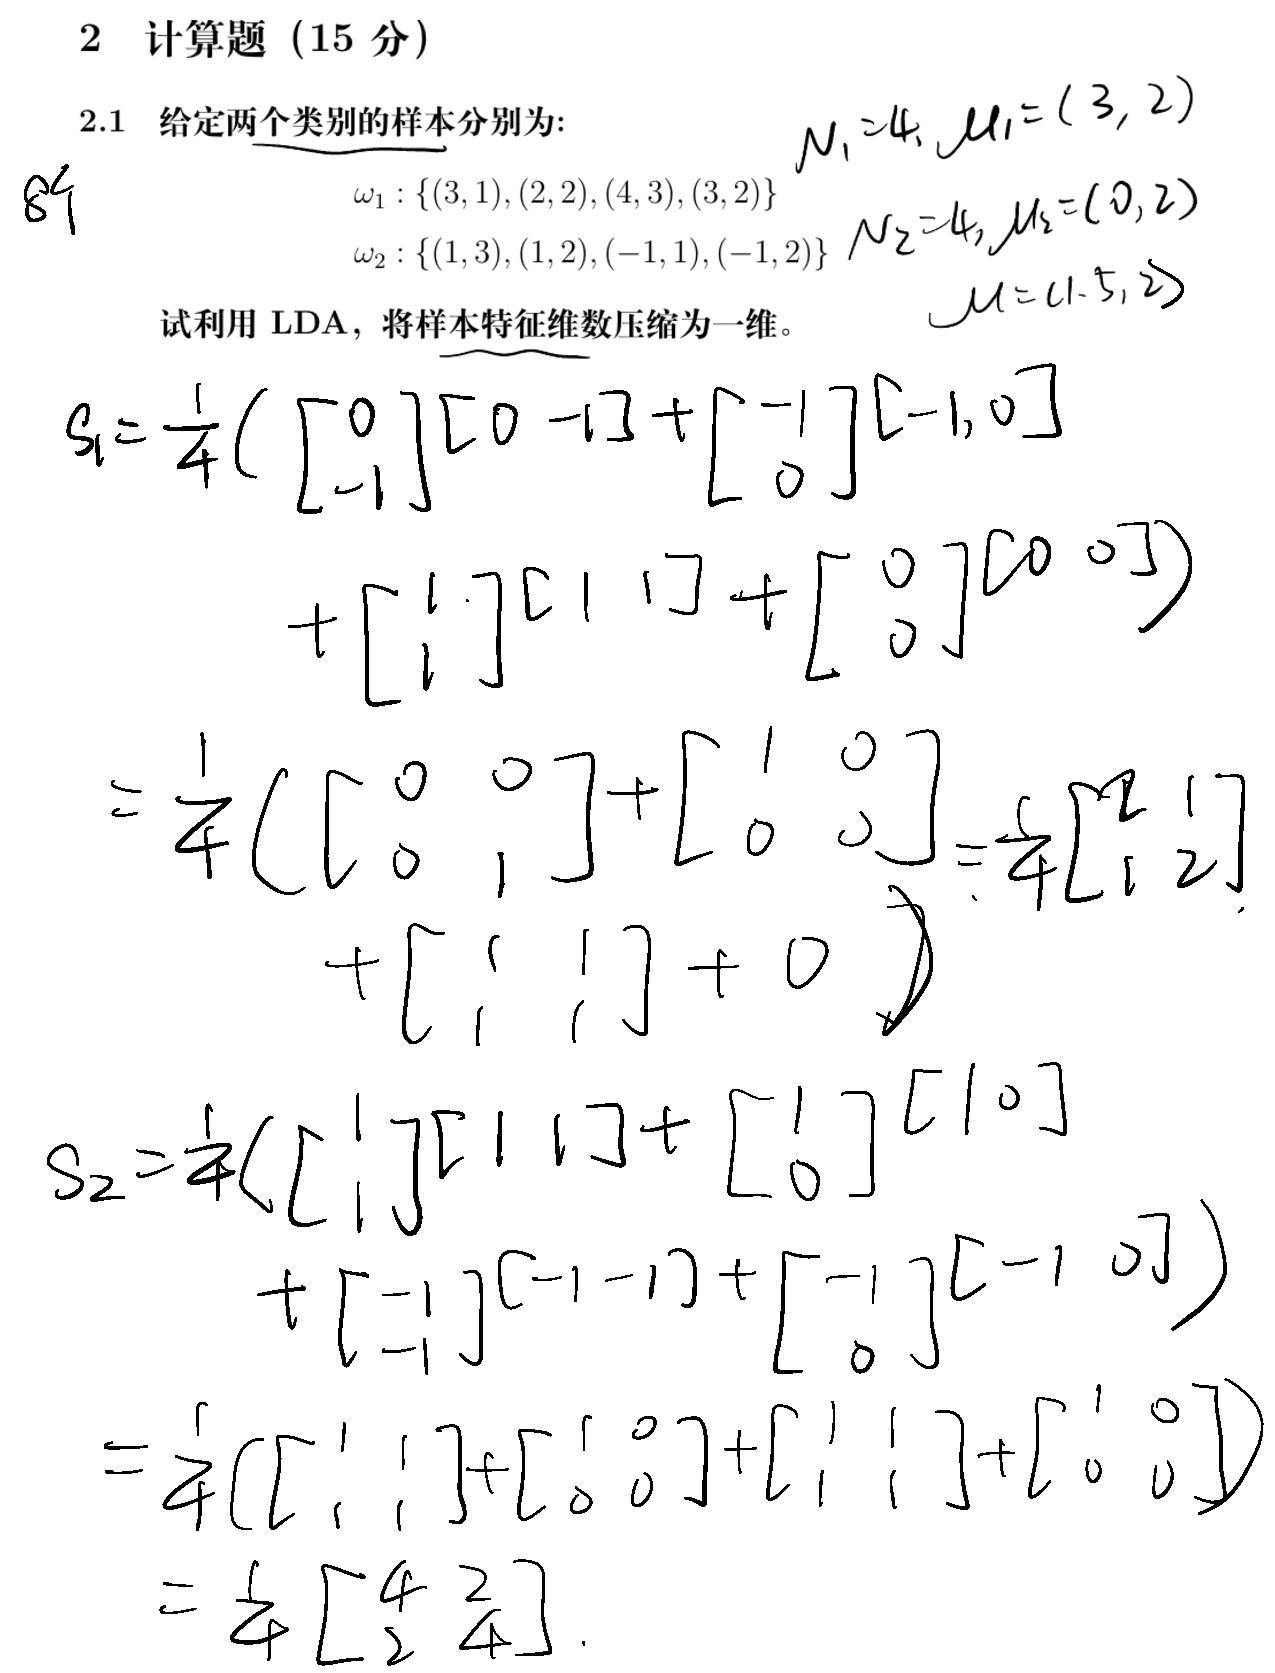
\includepdf[pages=-, scale=0.8, pagecommand={}]{myHW3.pdf}


\vspace{3mm}
\centerline{\textbf{\Large{编程部分}}}


\vspace{3mm}
% 请根据是否选择自选课题的情况选择“编程作业报告”或“自选课题进度汇报”中的一项完成
\section{编程作业报告}
% 请在此处完成编程作业报告

\end{document}



%%% Local Variables:
%%% mode: late\rvx
%%% TeX-master: t
%%% End:
